% \documentclass{article}
% \usepackage[utf8]{inputenc}
\documentclass{assignment format}
\usepackage{assignment}
\usepackage{bm}
\setcounter{section}{-1}
\setcounter{subsection}{-1}
\usepackage{amsmath, amsthm, amssymb}
\usepackage{enumerate}
\usepackage{enumitem}
\usepackage{kotex}
\usepackage{amsfonts}
\usepackage[dvipsnames]{xcolor}
\usepackage{enumitem}
\usepackage{url}
\usepackage{graphicx}
\usepackage{float} 
\usepackage{physics}
\usepackage{bbm}
\usepackage{caption}
\usepackage{minted}
\usepackage{todonotes}
\usepackage{relsize}
\usepackage{float}
\usepackage{blindtext}
\usepackage{multicol}
\newcommand{\note}[4][]{\todo[author=#2,color=#3,size=\scriptsize,fancyline,caption={},#1]{#4}} % default note settings, used by macros below.
\newcommand{\mrinmaya}[2][]{\note[#1]{mrinmaya}{blue!40}{#2}}

\usepackage[colorlinks=true]{hyperref}

\DeclareMathOperator*{\argmax}{arg\,max}

\newenvironment{answer}{
    {\bf Answer:} \begingroup\color{red}
}{\endgroup}%

\begin{document}

\makeheader{\textbf{Due on} Thursday Sep. 29, 2022 \\ by \textbf{3:30pm (before class)}}{Assignment 1: Word and Sentence Representation}
\begin{center}
%%%%%YOUR NAME HERE%%%%%

\fbox{%
  \parbox{\textwidth}{
  \begin{center}
\large\textbf{Honor Pledge for Graded Assignments}
\\ 
\\ 
   \large{ “I, YOUR NAME HERE , affirm that I have not given or received any unauthorized help on this assignment, and that this work is my own.”}
    \end{center}
}%
}
\end{center}
\def\showanswers{1}

\section{Instructions (4)}
\begin{itemize}
\item Total score cannot exceed 100 points. For example, if you score 95 points from non-bonus questions and 10 points are added from bonus questions, your score will be 100 points, not 105 points.
\item You can download the skeleton code file \href{https://raw.githubusercontent.com/yc-song/gsds-nlp-assignment-1/main/a1.zip}{HERE} 
\item You can download the TeX file \href{https://raw.githubusercontent.com/yc-song/gsds-nlp-assignment-1/main/a1(tex).zip}{HERE} 
\item Skeleton codes for problem 1, 2, 3, and 4 are at the directory \texttt{/skipgram}, \texttt{/fasttext}, \texttt{/sentence}, and \texttt{/tfidf} each. 
\item Run the \texttt{bash collect\_submission.sh} script to produce your 2022\_abcde\_coding.zip file. Please make sure to modify collect\_sumbssion.sh file before running this command. (\textbf{abcde} stands for your student id)
\item Modify this tex file into \texttt{2022\_abcde\_written.pdf} with your written solutions
\item Upload both \texttt{2022\_abcde\_coding.zip} and \texttt{2022\_abcde\_written.pdf} to etl website. \textbf{(4pts)}
\end{itemize}

%%%NOTE FOR MYSELF%%%


% 40000 ITERATION -> 20000
% list up python files to submit
% dataset 변경

\section{Understanding Skip-Gram (36)}

\subsection{Sofmax Loss Function}
Word representation by \textbf{Word2vec} is theoretically supported by  \textit{distributional hypothesis}\footnote{The hypothesis that words that occur in similar contexts have similar meanings.} In the example below, a `center' word \textit{banking} is surrounded by `outside' words \textit{turning, into, crises}, and \textit{as} when the context window length is 2.

\begin{figure}[h]
    \centering
    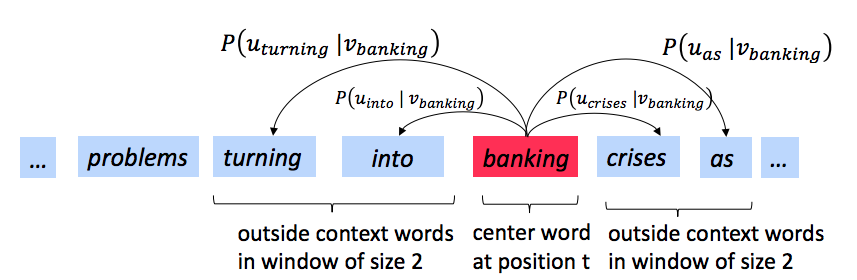
\includegraphics[width=0.6\textwidth]{word2vec.png}
    \caption{The skip-gram prediction model with window size 2}
    \label{fig:word2vec}
\end{figure}
The objective of training Skip-gram is to learn the conditioned probability distribution of outside word {O} given center word \textit{C}, $P(O=o|C=c)$. (i.e. the probability of the word o is an 'outside' word for word c)
The probability can be obtained by taking the softmax function over the inner product of word vectors as below:
\begin{equation}
 P(O=o \mid C=c) = \frac{\exp(\bm u_{o}^\top \bm v_c)}{\sum_{w \in \text{Vocab}} \exp(\bm u_{w}^\top \bm v_c)}
 \label{word2vec_condprob}
\end{equation}
where $u_o$ is the 'outside vector' representing outside word \textit{o}, and $v_c$ is the 'center vector' representing center word c. Be aware that outside and center vector representations of the same word are defined differently.

For the whole vocabulary, we can store outside vector $u_w$ and center vector $v_w$ in two matrices, $U$ and $V$ by columns. That is, the columns of $U$ are all the outside vectors $u_w$ and the columns of $V$ are all the center vectors $v_w$ for every $w \in Vocabulary$


% The true distribution $y$ is a one-hot vector with a 1 for the true outside word o, and 0 everywhere else. The predicted distribution $\hat{y}$ is the probability distribution $P(O|C=c)$ given by Skip-gram model in equation (\ref{word2vec_condprob}).

The loss for a single pair of words $c$ and $o$ is defined as:


\begin{equation}
 J_{\text{naive-softmax}}(\bm v_c, o, \bm U)=-\log P(O=o|C=c)= -\log\frac{\exp(u_{o}^\top v_c)}{\sum_{w \in \text{Vocab}} \exp( u_{w}^\top v_c)}=-u_o^T v_c+\log\sum_{w\in vocab}\exp(u_w^Tv_c)
\label{loss}
\end{equation}


To learn the correct center and outside vector by gradient descent, we need to compute the partial derivative of the outside and center word vectors. Partial derivative of $J_{\text{naive-softmax}}$ with respect to $v_c$ can be obtained as following:
\begin{equation}
\frac{\partial J}{\partial v_c}= -u_o^T+\frac{\sum_{i\in vocab} u_i^T\exp(u_i^Tv_c)}{\sum_{w\in vocab}\exp(u_w^Tv_c)}\\
=-u_o^T+\sum_{i\in vocab}P(O=i|C=c)u_i^T\\= -u_o^T+\sum_{w \in vocab}\hat{y}_wu_w^T\\
= -\mathbf{y}^TU^T+\hat{\mathbf{y}}^TU^T
\label{partial v_c}
\end{equation}where $\mathbf{y}$ is the one-hot vector which has 1 at the index of true outside word $o$ ($y_o=1$ and 0 for all other $i!=o$, $y_i=0$), and 0 everywhere else while $\hat{\mathbf{y}}$ stands for $P(O|C=c)$, a prediction made by Skip-gram model in equation (\ref{word2vec_condprob}).
\begin{enumerate}[label=(\alph*)]
	\item When is the gradient (\ref{partial v_c}) is zero? \textbf{(4pts)}
 %%%%%ANSWER FOR 1.1a%%%%%%
    \begin{answer}
    
    \end{answer}
    \item  If we update $v_c$ with this gradient, toward which vector is $v_c$ getting pulled to?  \textbf{(4pts)}
    \begin{itemize}
    \item \textbf{HINT}: The loss for a single pair of words $c$ and $o$ can be thought of as the cross-entropy between the true distribution \textbf{$y$} and the predicted distribution \textbf{$\hat{y}$} for a particular center word c and outside word o.
\begin{equation} 
\bm J_{\text{naive-softmax}}(\bm v_c, o, \bm U) = -\log P(O=o| C=c) =\\-\sum_{w \in vocab}y_w\log(\hat{y}_w)=-\log{\hat{y}_o}.
\label{naive-softmax}
\end{equation}

\end{itemize}
 %%%%%ANSWER FOR 1.1b%%%%%%
  \begin{answer}
    
    \end{answer}  
    \item Derive the partial derivatives of $J_{\text{naive-softmax}}$ with respect to the outside word vector matrix, $U$.
    \begin{itemize} 
\item \textbf{Note 1}: To get full credit, please write your answer in the form of $v_c, \mathbf{y}$, and $\hat{\mathbf{y}}$ and write the whole computation process. That is, the correct answer does not refer to other vectors but $v_c, \mathbf{y}$, and $\hat{\mathbf{y}}$. 
\item \textbf{Note 2}: Be careful about the dimensions of arrays and matrices. The final answer should have the same shape as U. (i.e. (vector length) $\times$ (vocabulary size)) 
\item\textbf{HINT}: Start from outside word vector $u_w$, which is the column vector of $U$. Then, dividing into two cases may help: when $w=o$ and $w \neq o$ \textbf{(6pts)}
\end{itemize}
%%%%%ANSWER FOR 1.1c%%%%%%
\begin{answer}

    \end{answer}
\end{enumerate}


\subsection{Negative Sampling Loss}
Now we shall consider the Negative Sampling loss, which is an alternative to the Naive Softmax loss.  Assume that $K$ negative samples (words) are randomly drawn from the vocabulary. For simplicity of notation we shall refer to them as $w_1, w_2, \dots, w_K$, and their outside vectors as $\bm u_{w_1}, \bm u_{w_2}, \dots, \bm u_{w_K}$. 
For a center word $c$ and an outside word $o$, the negative sampling loss function is given by:
\begin{equation}
\bm J_{\text{neg-sample}}(\bm v_c, o, \bm U) = -\log(\sigma(\bm u_o^\top \bm v_c)) - \sum_{s=1}^K \log(\sigma(-\bm u_{w_s}^\top \bm v_c))
\label{negsample}
\end{equation}
for a sample $w_1, \ldots w_K$, where $\sigma(\cdot)$ is the sigmoid function.
\begin{enumerate}[label=(\alph*)]
\item Compare the computational complexity of negative sampling with that of the softmax loss function presented in section 1.1. State the reason why negative sampling is computationally more efficient. \textbf{(6pts)}

%%%%%ANSWER FOR 1.2 a%%%%%%
\begin{answer}

    \end{answer}
\item Compute the partial derivatives of $\bm J_{\text{neg-sample}}$ with respect to $\bm v_c$, $\bm u_o$, and the $s^{th}$ negative sample $\bm u_{w_s}$. Please write your answers in terms of the vectors $\bm v_c$, $\bm u_o$, and $\bm u_{w_s}$, where $s \in [1, K]$.
 (within five lines)
\textbf{(6pts)}
%%%%%ANSWER FOR 1.2 b%%%%%%
\begin{answer}

    \end{answer}
\end{enumerate}
\subsection{Coding}
In this part, you will implement the Skip-Gram model and train word vectors with stochastic gradient descent (SGD). Before you begin, first run the following commands within the assignment directory in order to create the appropriate conda virtual environment. This guarantees that you have all the necessary packages to complete the assignment. You will be asked to implement the math functions above using the Numpy package at the root directory. 

\begin{minted}{bash}
    conda env create -f env.yml
    conda activate a1
\end{minted}

Once you are done with the assignment you can deactivate this environment by running:
\begin{minted}{bash}
    conda deactivate
\end{minted}
For each of the methods you need to implement, we included approximately how many lines of code our solution has in the code comments. These numbers are included to guide you. You don't have to stick to them, you can write shorter or longer code as you wish. If you think your implementation is significantly longer than ours, it is a signal that there are some \texttt{numpy} methods you could utilize to make your code both shorter and faster. \texttt{for} loops in Python take a long time to complete when used over large arrays, so we expect you to utilize \texttt{numpy} methods. The sanity checking function is provided to check if your code works well.
\newline
To run the code command below, please move your directory to \texttt{/skipgram}.
\begin{enumerate}[label=(\alph*)]
    \item We will start by implementing methods in \texttt{word2vec.py}. You can test a particular method by running \texttt{python word2vec.py m} where \texttt{m} is the method you would like to test. For example, you can test the naiveSoftmaxLossAndGradient method by running \texttt{python word2vec.py naiveSoftmaxLossAndGradient}. (Copy and paste it to your terminal)
        \begin{enumerate}[label=(\roman*)]
        \item Implement the softmax loss and gradient in the \texttt{naiveSoftmaxLossAndGradient} method. \textbf{(3pts)}
        \item Implement the negative sampling loss and gradient in the \texttt{negSamplingLossAndGradient} method. \textbf{(3pts)}
    \end{enumerate}
    \item When you are done, test your entire implementation by running \texttt{python word2vec.py}. Now we are going to load some real data and train word vectors with everything you just implemented! We are going to use The Recognizing Textual Entailment (RTE) dataset to train word vectors. (You can check out the raw datasets in the directory \texttt{./skipgram/utils/datasets/RTE}. There is no additional code to write for this part; just run \texttt{python run.py}.

    (\textbf{Note}: The training process may take a long time depending on the efficiency of your implementation and the computing power of your machine \textbf{(an efficient implementation takes around three to four hours)}. Please start your homework as soon as possible!)

    After 40,000 iterations, the script will finish and visualization for your word vectors will appear. It will also be saved as \texttt{word\_vectors.png} in your project directory. \textbf{Include the plot below} \textbf{(4pts)}
%%%%%ANSWER FOR 1.3 b%%%%%%
    
    \begin{answer}

    \end{answer}
\end{enumerate}
\section{FastText (28+4)}
\subsection{FastText Loss Function}
Let's move on to the FastText model.
Similar to the Skip-gram model, the loss function we are trying to optimize (for a single context word) is given as follows:
\begin{align*}
    \bm J(v_c, u_o, u_{w_s}) &= - \log(\sigma(s(v_c, u_o)))  - \sum_{s=1}^K \log(\sigma(-s(v_c, u_{w_s}))) \\
    s(w, u_o) &= \sum_{g \in G_w} z_g^T u_o
\end{align*}
We associate a vector representation $z_g$ to each character n-gram $g$. 
Make sure you understand how this expression is written using the sigmoid ($\sigma$) is similar to the one in the paper. 
Extending this to every outside word, we get the objective as:
\begin{align*}
    \bm J_{\text{FastText}}(w_c, w_{t-m}, w_{t-m+1} \dots w_{t+m}) = \sum_{\substack{-m\le j \le m \\ j\ne 0}} \bm J(w_t, w_c, N_K)
\end{align*}
The embeddings of the n-grams from the center words are from the  \textit{center} embeddings $V$ while the embeddings for the outside words are drawn from  \textit{outside word} embeddings $U$. 

\begin{enumerate}[label=(\alph*)]
    \item You train a Skip-gram model and a fastText model (with parameters as described in the paper) on a corpus of text. You train these models to have embeddings of size 128. Your corpus has 40000 unique words. Your model is upper-bounded by $2e6$ subword tokens. \\
    How many parameters are there in the Skip-gram model and FastText model? \textbf{(4pts)}\\ 
    \textbf{For more details, please refer to the papers:}
    \begin{itemize} 
\item \textbf{Skip-Gram}: \url{https://arxiv.org/pdf/1310.4546.pdf}
\item \textbf{FastText}: \url{https://arxiv.org/pdf/1607.04606.pdf}
\end{itemize} 
%%%%% Answer for 2.1-a %%%%%%
\begin{answer}
\end{answer}
    \item Calculate $\pdv{\bm J}{u_o}$  and $\pdv{\bm J}{u_{w_s}}$
    \textbf{(6pts)}
    \newline
%%%%% Answer for 2.1-b %%%%%%
\begin{answer}
\end{answer}
    \item Calculate  $\pdv{\bm J}{z_g}$
\textbf{(4pts)}%%%%% Answer for 2.1-c %%%%%%
    
\begin{answer}
    \end{answer}
    
\end{enumerate}

\subsection{Coding}

\begin{enumerate}[label=(\alph*)]
    \item We will start by implementing methods in \texttt{./fasttext} directory. After setting your python(or conda) environment as instructed on Problem 1. You can test a particular method by running \texttt{python word2vec.py m} where \texttt{m} is the method you would like to test. For example, you can test the negSamplingLossAndGradient method by running \texttt{python fasttext.py negSamplingLossAndGradient}. (Copy and paste it to your terminal)
    \newline
    To run the code command below, please move your directory to \texttt{/fasttext}.
        \begin{enumerate}[label=(\roman*)]
        \item Implement the negative sampling loss and gradient in the \texttt{negSamplingLossAndGradient} method in the \texttt{word2vec.py} of \texttt{./fasttext} directory. (\textbf{HINT}: Just copy and paste the code from the previous question. Be aware that the names of some arguments have changed.) \textbf{(3pts)}
        \item Implement \texttt{generate\_ngrams} function in the \texttt{utils/treebank.py} file. Sanity check by \texttt{python utils/treebank.py generate\_ngrams}. \textbf{(3pts)}
    \end{enumerate}
    \item When you are done, run the entire implementation by command \texttt{python run.py}. (check out you are in the right directory \texttt{./fasttext})

    (\textbf{Note}: The training process may take a long time depending on the efficiency of your implementation and the computing power of your machine \textbf{(an efficient implementation takes around two hours)}. Please start your homework as soon as possible!)

    After 20,000 iterations (which is shorter than word2vec), the script will finish and visualization for your word vectors will appear. It will also be saved as \texttt{word\_vectors.png} in your project directory. \textbf{Include the plot below} How is the plot different from the one generated earlier from Skip-Gram? \textbf{(4pts)}
%%%%%ANSWER FOR 2.2 b%%%%%%
    
    \begin{answer}

    \end{answer}
    \item What do you think are the advantages of a subword approach such as fastText compared to word2vec? (state within one line) \textbf{(4pts)}\\
%%%%%ANSWER FOR 2.2 c%%%%%%
    \begin{answer}

    \end{answer}
\item \textbf{(Bonus)} Can you think of a few examples where subword approach might hurt the embedding’s performance? (two or three examples are enough) \textbf{(4pts)}\\
%%%%%ANSWER FOR 2.2 d%%%%%%
    \begin{answer}

    \end{answer}
\end{enumerate}
\section{Vector Representation of Sentences (12+4)}
Based on word representation which we learned from Questions 1 and 2, we will represent sentences by averaging vectors of words consisting of sentences (Bag of words). Skeleton code is provided on \texttt{sentence/}\texttt{representing}\newline\texttt{\_sentence}\texttt{\_vectors.py} file. Every method and function is presented for you. What you are supposed to do is just run those codes and write down your answer.
\begin{enumerate}[label=(\alph*)]
\item Tokenization splits a sentence (string) into tokens, rough equivalent to words and punctuation. For example, to process the sentence 'I love New York', the given sentence needs to be tokenized to ['I', 'love', 'New', 'York']. Many NLP libraries and packages support tokenization, because it is one of the most fundamental steps in the NLP pipeline. However, there is no standard solution that every NLP practitioner agrees upon. Let's compare how different NLP packages tokenize sentences.
\newline
What is the main difference between two methods, \texttt{word\_tokenize} and \texttt{WordPunctTokenizer}? (state within one line) \textbf{(4pts)}
%%%%%ANSWER FOR 3 a%%%%%%
\begin{answer}
\end{answer}
\item Stop words are the words in a stop list which are filtered out (i.e. stopped) before or after processing of natural language data (text). Let's check out the English stopwords list of NLTK by running the code in the \texttt{representing\_sentence\_vectors.ipynb}.
\newline
After running the code and checking out the list, state \textbf{TWO} reasons why stopwords removal is useful in preprocessing. \textbf{(4pts)}
%%%%%ANSWER FOR 3 b%%%%%%
\begin{answer}
\end{answer}
\item 
Find three sentences where $s_1$ and $s_2$ have similar meanings and $s_1$ and $s_3$ have opposite meanings, while cosine distance between $(s_1, s_2)$ is longer than $(s_1, s_3)$  
As an example, $s_1$="I like everything of this movie. The only thing I do not like is the cast." is closer to $s_3$="I do not like everything of this movie. The only thing I like is the cast." than to $s_2$="I love all about this movie." in the vector space. Please find a different example that satisfies the above. Once you have found your example, please give a possible explanation for why this counter-intuitive result may have happened.
\textbf{(4pts)}

%%%%%ANSWER FOR 3 c%%%%%%
\begin{answer}

\end{answer}
\item \textbf{(Bonus)} What could we do beyond bag of words to resolve the issues presented at the problem (c)? Propose your own model that can represent sentences only using multi-layer perceptron (MLP) that can process variable-length sentences. Simply describe the idea with writing (and drawing) in a few lines. \textbf{(4pts)}
\newline
\textbf{(HINT:} if you know CNN, use MLP in similar manner)
\newline
%%%%%ANSWER FOR 3 d%%%%%%
\begin{answer}

\end{answer}
\end{enumerate}

\section{Document Retrieval (20+4)}
Information Retrieval involves the process of obtaining information from a system based on an information need. 
One example is to obtain documents relevant to a user query from a large corpus of documents. 
The vector space model models these documents as vectors that represent these documents. 
A query can be represented as another vector. 
We can now find similar documents to a query by using some form of distance in the vector space, like cosine similarity:

\begin{align*}
    \text{cosine similarity} = \text{cos}(\theta) = \frac{{\bf q}.{\bf d}}{\lVert {\bf q} \rVert \lVert {\bf d} \rVert }
\end{align*}
where ${\bf q}$ and ${\bf d}$ are the query and document vectors respectively. 

How are these vector space models built?
Let us represent a corpus of documents as a term-document matrix.
A term-document matrix is a mathematical matrix that describes the frequency of terms that occur in a collection of documents. In a document-term matrix, rows correspond to documents in the collection and columns correspond to terms. The entries in the matrix can be defined in different ways (we will describe a few variations in this assignment question).
A term document matrix allows for a way to index several documents against which a user query can be compared to fetch relevant documents.

Consider a corpus of documents:
\begin{verbatim}
I AM SAM
I LIKE SAM I AM
I LIKE GREEN EGGS AND HAM
\end{verbatim}

\subsection{Simple Word Counts}
You can answer the following questions. Skeleton code is presented at \texttt{tfidf/document\_retrieval.ipynb}. 
\begin{enumerate}[label=(\alph*)]
    \item Create a term document matrix using simple word counts (number of times a word appears in a document) for all the documents.  \textbf{(4pts)}
    %%%%%ANSWER FOR 4.1 a%%%%%%
        \begin{answer}
\begin{table}[H]
\centering
\label{tab:my-table}
\begin{tabular}{|l|l|l|l|l|l|l|l|l|}
\hline
     & I & AM & SAM & LIKE & GREEN & EGGS & AND & HAM \\ \hline
doc1 &   &    &     &      &       &      &     &     \\ \hline
doc2 &   &    &     &      &       &      &     &     \\ \hline
doc3 &   &    &     &      &       &      &     &     \\ \hline
\end{tabular}
\end{table}
    \end{answer}
    \item Using the vector space model and cosine similarity, find the closest document to the user query ``I LIKE EGGS" and their cosine similarity. \textbf{(4pts)}
    %%%%%ANSWER FOR 4.1 b%%%%%%
        \begin{answer}

    \end{answer}
    
    \item What are some issues you see of using counts to create the document vector? (one or two are enough.) \textbf{(4pts)}
    %%%%%ANSWER FOR 4.1 c%%%%%%

        \begin{answer}

    \end{answer}
\end{enumerate}
\subsection{TF-IDF}
One solution to this problem is to use the TF-IDF representation.
    TF-IDF involves multiplying the term frequency (which can be the raw counts) with an inverse document frequency (idf). 
    The inverse document frequency is a measure of how much information the word provides, i.e., if it is common or rare across all documents. 
     It is the logarithmically scaled inverse fraction of the documents that contain the word (obtained by dividing the total number of documents by the number of documents containing the term, and then taking the logarithm of that quotient).
     
     \begin{align*}
         \text{idf}(t) = \log_2(\frac{\text{Number of documents in the corpus}}{\text{Number of documents $t$ appears in}})
     \end{align*}\begin{enumerate}[label=(\alph*)]
         \item  Now instead of using the raw counts, use TF-IDF for each entry in the term-document matrix. Using the vector space model and cosine similarity find the closest document to the user query ``I LIKE EGGS" for the new index  \textbf{(4pts)}
             %%%%%ANSWER FOR 4.2 a%%%%%%

\begin{answer}
\begin{table}[H]
\centering
\label{tab:my-table}
\begin{tabular}{|l|l|l|l|l|l|l|l|l|}
\hline
     & I & AM & SAM & LIKE & GREEN & EGGS & AND & HAM \\ \hline
doc1 &   &    &     &      &       &      &     &     \\ \hline
doc2 &   &    &     &      &       &      &     &     \\ \hline
doc3 &   &    &     &      &       &      &     &     \\ \hline
query &   &    &     &      &       &      &     &     \\ \hline
\end{tabular}
\end{table}
    \end{answer}
	\item How does TF-IDF solve the issue quoted in 4.1? \textbf{(4pts)}
            %%%%%ANSWER FOR 4.2 b%%%%%%
    \begin{answer}

    \end{answer}
    \item \textbf{(Bonus)} Instead of using cosine similarity we could also use the L2 distance. Implement the code using L2 distance. Based on the result, state which similarity function (L2 or cosine) would work better here.   \textbf{(4pts)}
        %%%%%ANSWER FOR 4.2 c%%%%%%
            \begin{answer}

    \end{answer}

\end{enumerate}

\end{document}
